\documentclass{article}
\usepackage{graphicx}
\title{ECE 1895 - ASSIGNMENT 1 REPORT (SECOND ATTEMPT)}
\author{Yinhao Qian}
\begin{document}
	\maketitle
	If pictures are obscure, they can be found from /LATEX. 
	Calculation source codes can be found under /MATLAB.
	Schematics can be found under /LTSPICE.
	\section*{Values selected:}
	According to the data sheet and and the relationships between resistors and periods, minimizing $R_A$ yields $t_h=t_l$. I selected the following values because such resistors are common, and making sure $R_A$ is very small compared to $R_B$:
	\[R_A=100\Omega\]
	\[R_B=10K\Omega\]
	\begin{verbatim}
		%Inputs:
		val_RA = 0.1e3;
		val_RB = 10e3;
		val_pRan = [20e-6,500e-6]; %period range
		%Calculations:
		val_CRan = val_pRan/(0.693*(val_RA+2*val_RB))
	\end{verbatim}
	\[C_2\subset(1.4358nF,35.8956nF)\]
	Picking a common capacitance values:
	\[C_2=10nF=0.01\mu F\]
	All other capacitors and resistors have no effect on the period, so I'll leave them unchanged from the data sheet. \textbf{I have removed the load resistor from the schematic as per the requirement.} For the source voltage,however, since no peak voltages are specified as per the requirements, I'll select an arbitrary source voltage:
	\[V_{CC}=10V\]
	All other required calculations are as follows:
	\begin{verbatim}
		val_C = 10e-9;
		val_peri = 0.693*(val_RA+2*val_RB)*val_C %period
		val_freq = 1.44/((val_RA+2*val_RB)*val_C) %frequency
		val_oddc = val_RB/(val_RA+2*val_RB) %output driver duty cycle
		val_owdc = 1 - val_RB/(val_RA+2*val_RB) %output waveform duty cycle
		val_lthr = val_RB/(val_RA+val_RB) %low-to-high ratio
	\end{verbatim}
	Results:
	\[\mbox{Period}=139.293\mu s\]
	\[\mbox{Frequency}=7.164KHz\]
	\[\mbox{Output Driver Duty Cycle}=49.75\%\]
	\[\mbox{Output Waveform Duty Cycle}=50.25\%\]
	\[\mbox{Low-to-high Ratio}=99.01\%\]
	\section*{Schematics}
	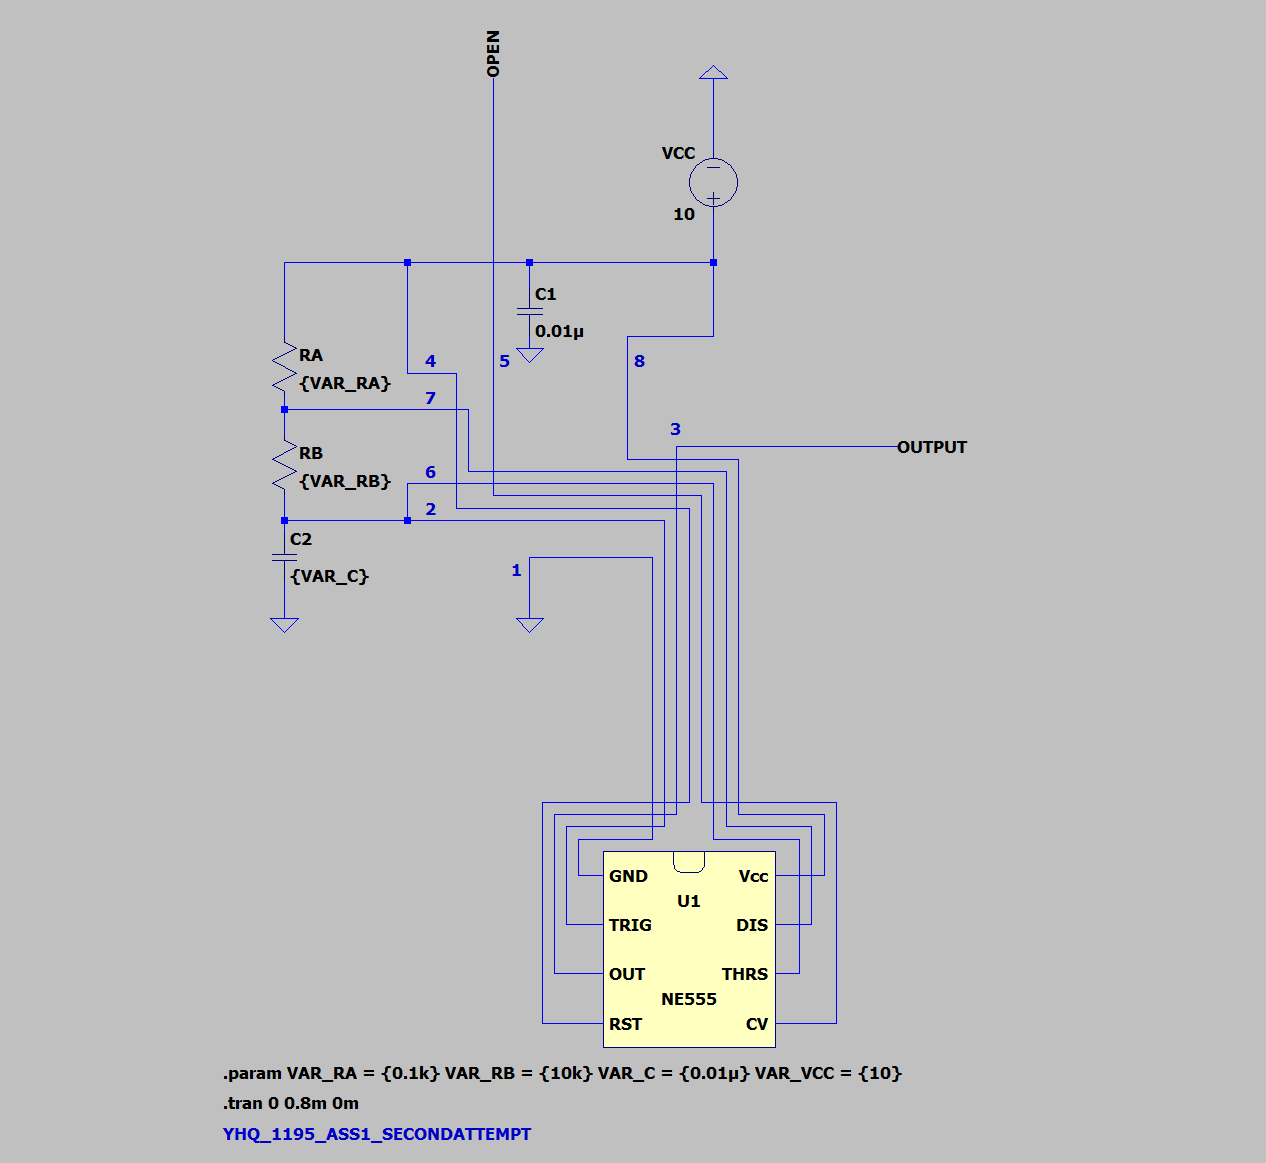
\includegraphics[width=\columnwidth]{schmatics.PNG}
	\section*{Simulations}
	Note that the period corresponds with what we desires.
	
	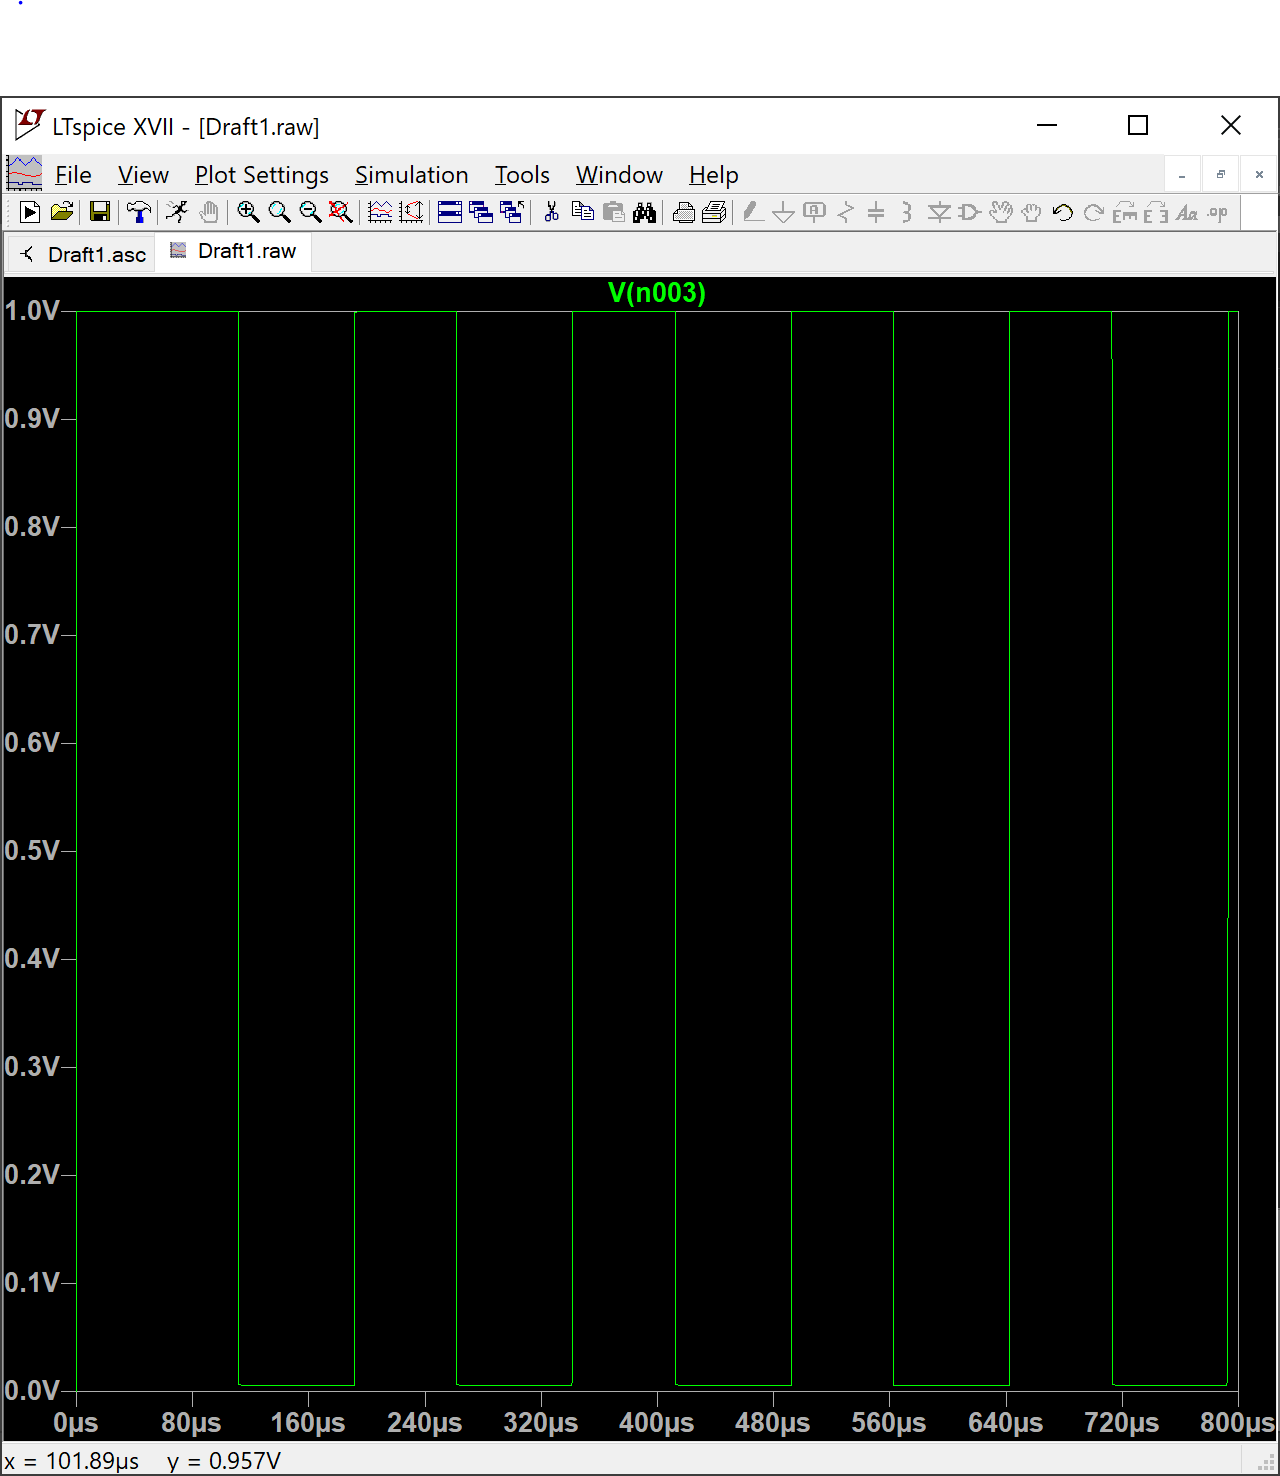
\includegraphics[width=\columnwidth]{waveform.PNG}
	
\end{document}